%!TEX TS-program = xelatex
%!TEX encoding = UTF-8 Unicode

\documentclass[12pt]{extarticle}
% extarticle is like article but can handle 8pt, 9pt, 10pt, 11pt, 12pt, 14pt, 17pt, and 20pt text

\def \ititle {Joint Action without Shared Intention}
\def \isubtitle {}
\def \iauthor {Stephen A. Butterfill}
\def \iemail{s.butterfill@warwick.ac.uk}
\date{}

\input{$HOME/Documents/submissions/preamble_steve_handout}



\begin{document}

\begin{multicols}{3}

\setlength\footnotesep{1em}

% \bibpunct{}{}{;}{s}{}{,}  %use superscript TICS style bib

\bibliographystyle{newapa} %apalike

\maketitle
%\tableofcontents



A joint action is a goal-directed action, or something resembling one, comprising two or more agents' goal-directed activities. 

`the unique aspects of human cognition ... were driven by, or even constituted by, social co-operation'
\citep[p.\ 1]{Moll:2007gu}.

`perception, action, and cognition are grounded in social interaction%
% … functions traditionally considered hallmarks of individual cognition originated through the need to interact with others
' \citep[p.\ 103]{Knoblich:2006bn}.

\section{First Half: collective goals}
What is the relation between a joint action and the goal (or goals) to which it is directed?

`I take a collective action to involve a collective intention.'  \citep[p.\ 5]{Gilbert:2006wr}.

`the key property of joint action lies in its internal component \ldots \ in the participants’ having a ``collective'' or ``shared'' intention.' \citep[pp. 444-5]{alonso_shared_2009}.

`Shared intentionality is the foundation upon which joint action is built.' \citep[p.\ 381]{Carpenter:2009wq}

`it is precisely the meshing and sharing of psychological states \ldots \ that holds the key to understanding how humans have achieved their sophisticated and numerous forms of joint activity'
\citep[p.\ 369]{Call:2009fk}

\begin{center}
  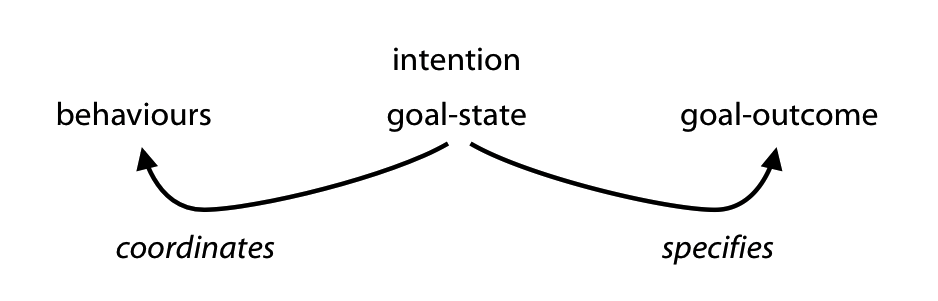
\includegraphics[width=0.3\textwidth]{standard_story.png}
\emph{Figure}: The standard story for individual action.
\end{center}



\textbf{Shared intention: necessary conditions ...}


- \emph{\textbf{awareness of joint-ness}} at least one of the agents knows that they are not acting individually; she or they have `a conception of themselves as contributors to a collective end.' \citep[p.\ 10]{Kutz:2000si}

- \emph{\textbf{awareness of others' agency}}  at least one of the agents is aware of at least one of the others as an intentional agent.

- \emph{\textbf{awareness of others' states or commitments}} at least one of the agents who are F-ing is aware of, or has individuating beliefs about, some of the others' intentions, beliefs or commitments about F.

\textbf{Distributive goal}.  The \emph{distributive goal} of two or more agents' activities is G: each agent's activities are individually directed to G.

\textbf{Collective goal}.  The \emph{collective goal} of a joint action is G:
(a) each agent’s activities are individually directed to G (i.e. G is a distributive goal);
(b) the agents’ activities are coordinated; and 
(c) G would normally occur partly as a consequence of this coordination, or would normally be partly constituted by it






\section{Second Half: shared goals}
What is the minimum we can add to the notion of collective goal in order to capture some joint actions with potentially novel goals which are voluntary with respect to their joint-ness?


\textbf{Shared goal}.  The \emph{shared goal} of two or more agents' activities is G: (a) G is a collective goal of their activities; (b) each agent expects each of the other agents to perform activities directed to G; and (c) each agent expects G to occur as a common effect of all their goal-directed actions, or to be partly constituted by all of their goal-directed actions.



\textbf{Bratman's shared intentions}

The functional role of shared intentions is to: 
(i) coordinate activities; (ii) coordinate planning; and (iii) provide a framework to structure bargaining \citep[p.\ 99]{Bratman:1993je}

For you and I to have a shared intention that we J it is sufficient that: `(1)(a) I intend that we J and (b) you intend that we J; (2) I intend that we J in accordance with and because of la, lb, and meshing subplans of la and lb; you intend that we J in accordance with and because of la, lb, and meshing subplans of la and lb; (3) 1 and 2 are common knowledge between us' \citep[View 4]{Bratman:1993je}


`each agent does not just intend that the group perform the […] joint action. Rather, each agent intends as well that the group perform this joint action in accordance with subplans (of the intentions in favor of the joint action) that mesh' \citep[p.\ 332]{Bratman:1992mi}

`philosophers ... postulate complex intentional structures that often seem to be beyond human cognitive ability in real-time social interactions.'
\citep[p.\ 2022]{Knoblich:2008hy}



Why do we need states which are neither collective goals nor shared intentions?  Some joint actions are both voluntary with respect to their jointness (so collective goals are not enough) and also spontaneous, requiring real-time coordination (so shared intention is too much).



\section{Application}
`regular participation in cooperative, cultural interactions during ontogeny leads children to construct uniquely powerful forms of cognitive representation.'
\citep[pp.\ 2-3]{Moll:2007gu}

`As in previous theoretical work […], we use here a modified version of Bratman’s (1992) definition of `shared cooperative activities'.' \citep[p.\ 3]{Moll:2007gu}


\textbf{your-goal-is-my-goal}: (1) We are about to engage in some joint action; (2) I am not about to change my goal; therefore (3) The others will each individually perform actions directed to my goal.


`to understand pointing, the subject needs to understand more than the individual goal-directed behaviour. She needs to understand that ... the other attempts to communicate to her ...  and ... the communicative intention behind the gesture'
(Moll \& Tomsello 2007)

`the adult’s social cues conveyed her communicative intent, which in turn encouraged the child to 'see through the sign'.'
\citep[p.\ 118]{leekam_adults_2010}

\footnotesize 
\bibliography{$HOME/endnote/phd_biblio}

\end{multicols}

\end{document}